\chapter{Triangulácia}

Usporiadanú trojicu množín $(V, E, F)$, kde $V$ je množina vrcholov daná ich súradnicami, 
$E$ je množina neorientovaných hrán daná 
dvojicou vrcholov z $V$ a $F$ je množina stien daných $n$-ticou vrcholov z $V$, kde $n \geq 3$, 
nazývame mesh.

V prípade, že všetky steny sú dané trojicou vrcholov, nazývame tento mesh trianguláciou.

Trianguláciou implicitného povrchu nazývame aproximáciu tohto povrchu trojuholníkovým meshom.

Podľa článku \textit{Adaptive implicit surface polygonization using marching triangles} \cite{akkouche2001adaptive}
vhodná triangulácia by mala spĺňať viacero podmienok. Vygenerovaný mesh by mal byť konzistentný, 
teda bez dier alebo rozpojených vrcholov, hrán alebo stien. Na obrázku \ref{obr:torus_holes}
môžeme vidieť ako vyzerá nekonzistentná triangulácia torusu, kdežto na obrázku \ref{obr:torus_no_holes}
sa nachádza vhodná triangulácia bez dier. 

\begin{figure}
    \centerline{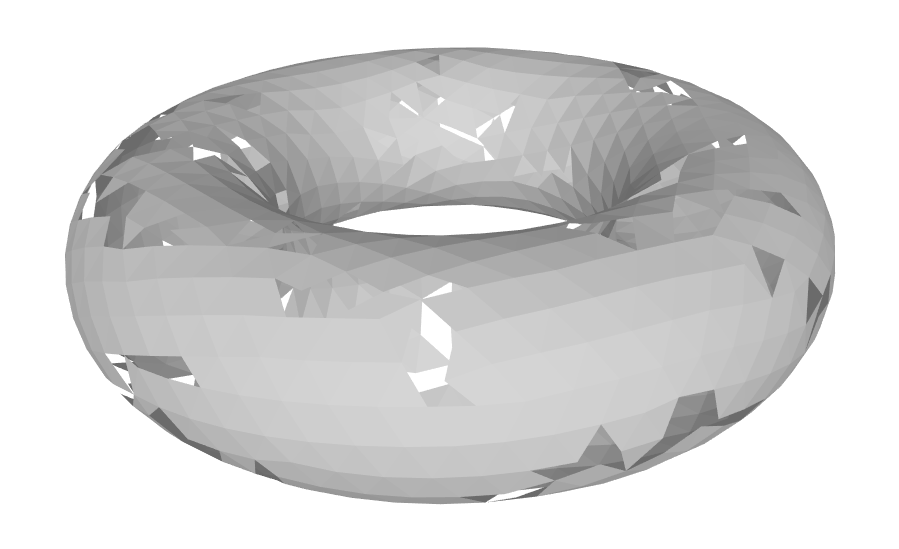
\includegraphics[width=0.8\textwidth]{images/torus_holes}}
    \caption[Nekonzistentná triangulácia torusu s dierami]{Nekonzistentná triangulácia torusu s dierami}
    %id obrazku, pomocou ktoreho sa budeme na obrazok odvolavat
    \label{obr:torus_holes}
\end{figure}

\begin{figure}
    \centerline{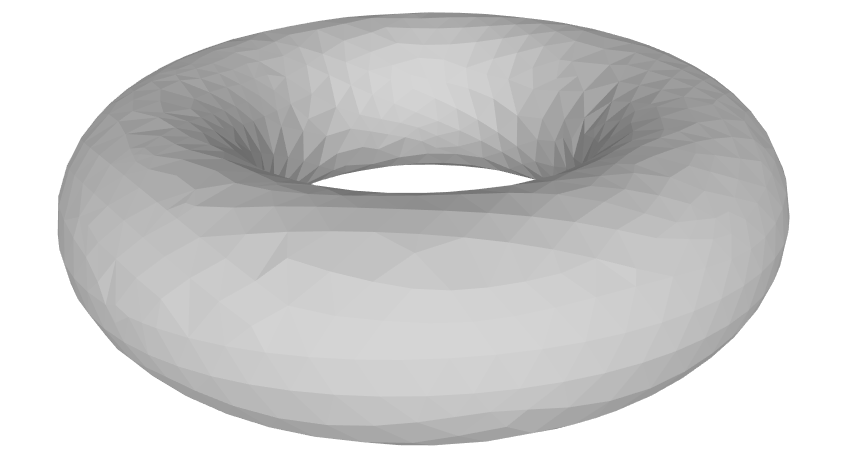
\includegraphics[width=0.8\textwidth]{images/torus_no_holes}}
    \caption[Konzistentná triangulácia torusu bez dier]{Konzistentná triangulácia torusu bez dier}
    %id obrazku, pomocou ktoreho sa budeme na obrazok odvolavat
    \label{obr:torus_no_holes}
\end{figure}

Ďalej by vzniknutá triangulácia mala byť topologicky homeomorfná 
so zadaným implicitným povrchom. Aproximácia by mala byť dostatočne presná a trojuholníky by mali 
byť čo najpravidelnejšie. Naviac triangulácia povrchu by sa mala prispôsobiť zakriveniu povrchu,
teda mala by vyprodukovať menšie trojuholníky v miestach s väčším zakrivením povrchu a naopak väčšie
trojuholníky v miestach s menším zakrivením.

Na tringuláciu implicitného povrchu sa používa množstvo rôznych prístupov, avšak nie každá metóda
dokáže vyprodukovať trianguláciu spĺňajúcu všetky kritéria, ktoré sme popísali. Na druhú stranu, 
presnejšie algoritmy, ktoré dokážu vyprodukovať kvalitné meshe potrebujú viac výpočtov a preto
trvajú dlhšie. 

K najrýchlejším metódam triangulácie implicitnej funkcie patria takzvané \textit{Space docomposition}
prístupy, ktoré delia priestor obsahujúci plochu na menšie bunky, napríklad kocky alebo štvorsteny.
Následne pomocou znamienka implicitnej funkcie sa vyhodnotí, či sa vrcholy buniek nachádzajú pod povrchom 
alebo nad ním. Pomocou numerických metód sa vypočítajú približné priesenčníky hrán týchto buniek s 
implicitnou funkciou a použijú sa vyhľadávacie tabuľky na zistenie triangulácie povrchu v danej bunke. 
To, že tieto metódy patria k najrýchješím nám napovedá, že nebudú príliš presné. Mnoho vedcov sa
však zameralo na tieto rýchle algoritmy a pomocou následného spracovania triangulácie sa im 
podarilo upraviť dané meshe na kvalitnejšie. Medzi najznámejšie \textit{Space docomposition} algoritmy
patrí \textit{Marching Cubes} \cite{lorensen1987marching} a \textit{Marching Tetrahedra} \cite{doi1991efficient}.

Ku kvalitnejším, avšak pomalším prístupom patria takzvané \textit{Surface tracking} prístupy.
Tieto algoritmy sa začínajú v bode ležiacom na povrchu (alebo dostatočne blízko povrchu) a 
postupne sledujú povrch a vytvárajú polygóny. Tu sa vyskytuje jedna z nevýhod implicitne zadaného
povrchu - zistiť bod ležiaci na povrchu je ťažšie ako pri explicitnom vyjadrení. Medzi najznámejšie 
\textit{Surface tracking} algoritmy patrí \textit{Marching Triangles} \cite{hilton1996marching}.



\subsection{Delaunayova triangulácia}

\begin{note}
    (difeomorfizmus)

    Pod difeomorfizmom medzi dvoma diferencovateľnými 3D manifoldmi $\mathbf{A}$ a $\mathbf{B}$ 
    môžeme rozumieť existenciu zobrazenia z $\mathbf{A}$ do $\mathbf{B}$, pričom toto zobrazenie 
    je invertibilné a spojite diferencovateľné. 
\end{note}

V tejto časti sa budeme venovať lokálnej podmienke pre potenciálny trojuholník, ktorý chceme pridať do 
výslednej triangulácie. Táto podmienka nám zaistí neprekrývajúce sa trojuholníky a teda topologickú 
ekvivalenciu implicitného povrchu a vytvorenej meshe.

Podľa článku \textit{Marching triangles: Delaunay implicit surface triangulation} \cite{hilton1997marching} 
\textit{3D Delaunayova triangulácia} ľubovoľnej množiny bodov $X\in \mathbb{R}^3$ je 
zložená zo štvorstenov takých, že pre každý z nich existuje guľa prechádzajúca cez každý z vrcholov 
štvrorstenu, ktorá neobsahuje žiadne iné body z $X$. V prípade, že body $X$ ležia na \textit{3D manifolde} 
v článku \textit{Geometric structures for three-dimensional shape representation} 
\cite{boissonnat1984geometric} odvodil \textit{J.D.Boissonnat} nasledujúcu vlastnosť. Trojuholník
lokálne difeomorfný s 3D manifoldom je v \textit{3D Delaunayovej triangulácii} ak spĺňa 
\textit{Delaunayovu vlastnosť}:

\begin{definition}
    (Delaunay face property)

    Trojuholník $\mathbf{T}$ je stenou v 3D Delaunayovej triangulácii množiny vrcholov 
    $\mathbf{X}\in \mathbb{R}^3$, ak existuje guľa prechádzajúca cez vrcholy trojuholníka 
    $\mathbf{T}$ a v tejto guli sa nenachádza žiadny ďalší vrchol z $\mathbf{X}$. 
\end{definition}

Príklad trojuholníka $T$, ktorý spĺňa \textit{Delaunayovu vlastnosť} môžeme vidieť na obrázku 
\ref{obr:delaunay_face_property}. V guli predchádzajúcej cez vrcholy trojuholníka $T$ 
sa nenachádza žiadny vrchol z množiny vrcholov.

\begin{figure}
    \centerline{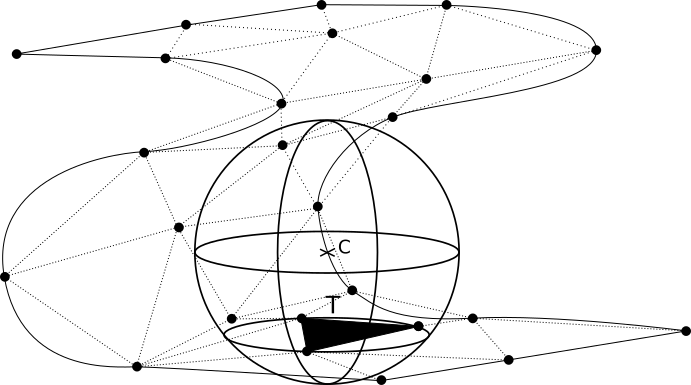
\includegraphics[width=0.6\textwidth]{images/delaunay_face_property}}
    \caption[\cite{hilton1996marching} Trojuholník $T$ spĺňa Delaunayovu vlastnosť]{\cite{hilton1996marching} Trojuholník $T$ spĺňa Delaunayovu vlastnosť}
    %id obrazku, pomocou ktoreho sa budeme na obrazok odvolavat
    \label{obr:delaunay_face_property}
\end{figure}

Ak túto vlastnosť spĺňajú všetky trjuholníky z polyhedronu, ktorý je difeomorfný so zadaným 
\textit{3D manifoldom}, tak je tento polyhedron Delaunayovou trianguláciou zadaného povrchu pre 
množinu bodov $\mathbf{X}$.

\textit{3D Delaunayova triangulácia} je analógom k \textit{2D Delaunayovej triangulácii}, pričom
body z množiny $\mathbf{X}$ ležia na 3D povrchu namiesto 2D roviny.

V článku \textit{Marching triangles: Delaunay implicit surface triangulation} \cite{hilton1997marching}
autori odvodili vhodnú podmienku na pridanie trojuholníka do meshe.

\begin{definition}
    (Delaunay constraint)

    Nech trojuholník $\mathbf{T}(x_i, x_j, x_{new})$ sa skladá z hraničnej hrany meshu $\mathbf{M}$ 
    $\mathbf{e}(x_i, x_j)$ a nového vrchola $x_{new}$. Tento trojuholník môžeme pridať do 
    $\mathbf{M}$ iba vtedy ak sa z doterajšej 
    množiny vrcholov žiadny vrchol, ktorý je súčasťou trojuholníka s rovnakou orientáciou ako 
    $\mathbf{T}$ nenachádza vnútri gule prechádzajúcej cez vrcholy $x_i, x_j, x_{new}$ so stredom 
    v bode C, kde C je stred opísanej kružnice trojuholníka $\mathbf{T}$. Pod rovnakou orientáciou 
    trojuholníkov $T_1$ a $T_2$ myslíme podmienku kladného skalárneho súčinu ich normál, teda 
    $\overrightarrow{\rm n_1} \cdot \overrightarrow{\rm n_2} > 0$.
\end{definition}




\subsection{Marching Cubes}

Algoritmus \textit{Marching Cubes} \cite{lorensen1987marching} patrí k najznámejším algoritmom používaným
na trianguláciu implicitného povrchu. Prvý krát bol prezentovaný v roku 1987. Patrí k najrýchlejším
algoritmom avšak výsledok postráda mnoho kritérií kvality triangulácie. 

---Toto chcem dať asi niekde do úvodu !TODO!


Primárna motivácia na vytvorenie algoritmu bola najmä vizuálizácia získaných dát napríklad z CT alebo MRI skenov 
využívaná v medicíne. Dnes majú vizualizácie implicitných povrchov oveľa širšie využitie.

Prístup \textit{rozdeľuj a panuj} spočíva rozdelení zložitejšieho problému na podproblémy, 
ktoré sa dajú jednoduchšie riešiť a následne tieto riešenia spojí do jedného.

Tento prístup sa rozhodli využiť aj autori algoritmu \textit{Marching Cubes}. Rozdelenie problému
spočíva v podrozdelení priestoru, v ktorom sa nachádza zadaný povrch na kocky so zvolenou dĺžkou
hrany. Následne sa pre každú kocku vypočíta, ktoré vrcholy sa nachádzajú pod povrchom (alebo na ňom) 
a ktoré nad povrchom. Keďže každá kocka má 8 vrcholov a každý vrchol môže nadobudnúť hodnotu $1$, ak sa 
nachádza pod povrchom alebo na ňom, alebo hodnotu $0$, ak sa nechádza nad povrchom, exisuje práve 
$2^8 = 256$ možností. Vďaka symetriám sa však autorom podarilo znížiť tento počet len na 14 rôznych možností.
Pre tieto možnosti vytvorili tabuľku, kde pomocou 8 bitového binárneho čísla označujúceho charakteristiku
kocky vyhľadávali dané triangulácie. Zredukovanú vyhľadávaciu tabuľku môžeme vidieť na obrázku \ref{obr:}

\begin{figure}
    \centerline{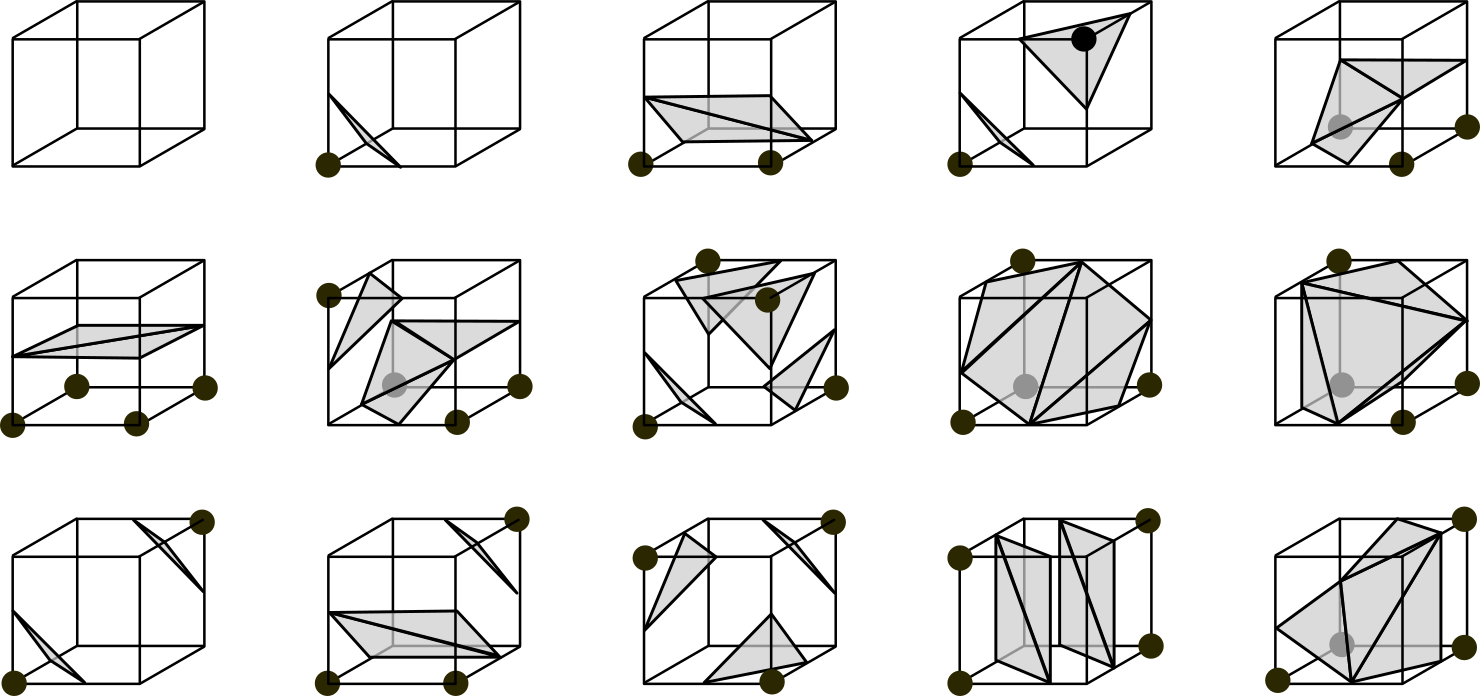
\includegraphics[width=0.95\textwidth]{images/lookup_table}}
    \caption[Zredukovaná vyhľadávacia tabuľka \cite{smistad2012real} pre metódu \textit{Marching Cubes}]{Zredukovaná vyhľadávacia tabuľka \cite{smistad2012real} pre metódu \textit{Marching Cubes}}
    %id obrazku, pomocou ktoreho sa budeme na obrazok odvolavat
    \label{obr:lookup_table}
\end{figure}

Približná poloha priesečníka s hranou kocky sa dá vypočítať napríklad pomocou lineárnej inerpolácie, avšak 
dajú sa použiť aj presnejšie, avšak pomalšie, interpolácie vyšších rádov. Najrýchlejšia avšak najmenej presná
možnosť je zvoliť ako priesenčník stred hrany kocky.

Analóg tejto metódy pre $2D$ môžeme vidieť na obrázku \ref{obr:marching_cubes}. V tomto prípade delíme rovinu na štvorce, 
vypočítame vrcholy nachádzajúce sa vnútri alebo na hranici. Tieto vrcholy sú na obrázku znázornené 
červenou farbou. V tomto prípade sú za priesenčníky zvolené stredy hrán znázornené modrou farbou. 
Pre $2D$ prípad existuje len $2^4 = 16$ možností, avšak aj tento počet sa dá vďaka symetrám zredukovať.


\begin{figure}
    \centerline{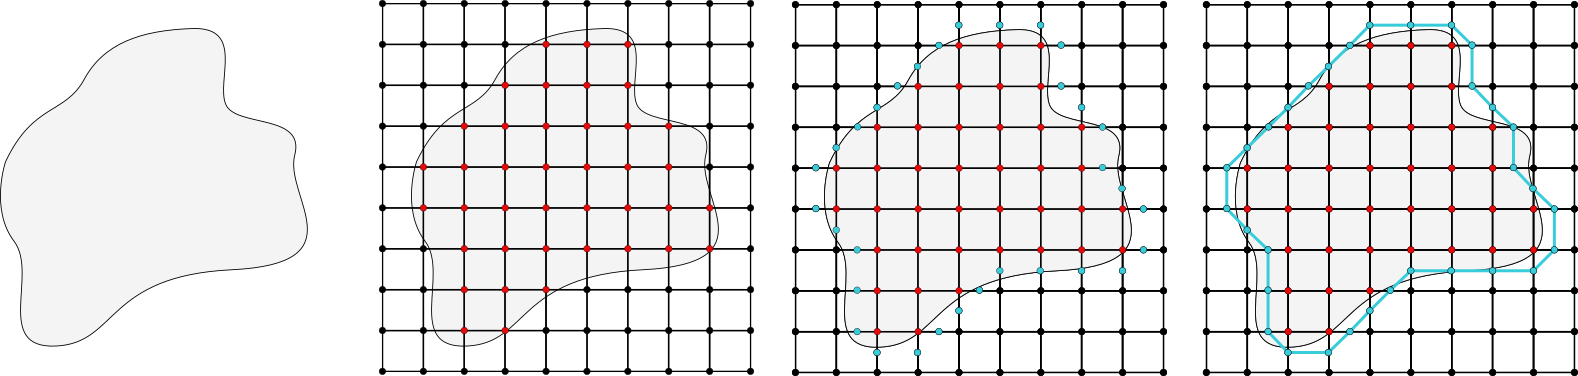
\includegraphics[width=0.95\textwidth]{images/marching_cubes}}
    \caption[Analóg metódy \textit{Marching Cubes} pre $2D$]{Analóg metódy \textit{Marching Cubes} pre $2D$}
    %id obrazku, pomocou ktoreho sa budeme na obrazok odvolavat
    \label{obr:marching_cubes}
\end{figure}

Táto metóda však mala problémy s jednoznačnosťou 

Výstupom algotitmu sú okrem triangulácie aj normály vo vrcholoch triangulačných trojuholníkov vypočítané pomocou lineárnej
interpolácie normalizovaného gradientu získaného pomocou \textit{centrálnej diferencie} vo vrcholoch prerozdelených kociek. 
Tieto normály sa používajú najmä na čo najpresnejšie tieňovanie triangulácie.


\subsection{Marching Triangles}

Algortimus \textit{Marching Triangles} \cite{hilton1996marching} patrí do skupiny algoritmov založených na takzvanom 
sledovaní povrchu. Prvý krát bol prezentovaný v roku 1996. Oproti algoritmu \textit{Marching Cubes} je pomalší, avšak
produkuje kvalitnejšiu trianguláciu. 

Algoritmus začína v počiatočnom bode na povrchu plochy. Následne vytvorí prvý trojuholník na povrchu a hrany vzniknutého 
trojuholníka vloží do zoznamu hraničných hrán. 
Opakujúc sériu krokov postupne zväčšuje trianguláciu. V každom z týchto krokov zo zoznamu vyberie jednu hranu $E$. 
Táto hrana susedí práve s jedným trojuholníkom. V rovine susedného trojuholníka vytvorí kolmicu na hranu $E$
(podľa \ref{obr:new_vertex}) a následne na nej bod $V$ v nejakej vzdialenosti $k$. 

\begin{figure}
    \centerline{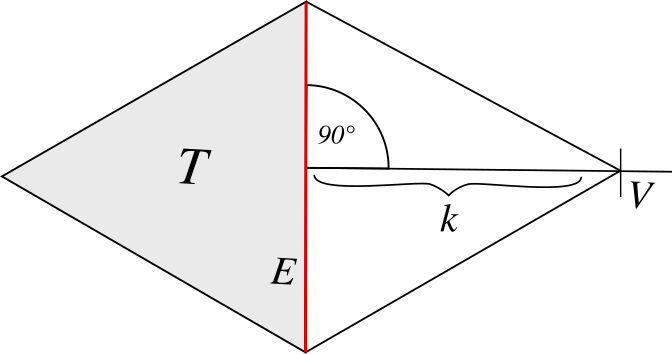
\includegraphics[width=0.6\textwidth]{images/new_vertex}}
    \caption[Vytváranie nového vrcholu $V$ v rovine susedného trojuholníka]{Vytváranie nového vrcholu v rovine susedného trojuholníka}
    %id obrazku, pomocou ktoreho sa budeme na obrazok odvolavat
    \label{obr:new_vertex}
\end{figure}

Vzdialenosť $k$ môže byť daná fixne alebo môže mať premenlivú veľkosť, v pôvodnom algoritme je táto vzdialenosť fixná. 
Následne sa tento bod pomocou numerických metód sprojektuje na povrch a overí sa \textit{Delaunayova podmienka} pre novovzniknutý 
trojuholník. 
Ak trojuholník spĺňa \textit{Delaunayovu podmienku}, pridá sa do triangulácie. V opačnom prípade sa snažíme vytvoriť iný trojuholník 
skladajúci sa z pôvodnej hrany a vrcholov, ktoré sú susedné k vrcholom tejto hrany. V prípade, že aj tieto trojuholníky nespĺňajú 
\textit{Delaunayovu podmienku}, pokúsime sa vytvoriť trojuholník s hraničným vrcholom už existujúcej triangulácie ktorý pretína
guľu kontrolujúcu $Delaunayovu podmienku$, ak taký existuje. Ak ju však ani tento trojuholník nesplní, testovanie danej hrany sa skončí.

Ak sa v danom kroku algoritmu pridá nejaký trojuholník do triangulácie, tak odoberieme hranu, s ktorou sme pracovali zo zoznamu a 
vložíme do nej novovytvorené hrany nachádzajúce sa na hranici.

Tento postup sa opakuje pokiaľ existujú neskontrolované hrany na hranici triangulácie.

\newpage

\section{Singulárne body a krivky}

Singulárne body implicitne danej funkcie sú také body, kde $\nabla F(x, y, z) = 0$. Tieto body nemusia byť nutne izlované, 
v tom prípade hovoríme o singulárnych krivkách. 

Singulárne body a krivky sa vyskytujú napríklad pri CSG modelovaní.

\medskip

!TODO! obrázok singulárnej krivky a bodu, ukážka funkcie v ktorej sa vyskytuje singulárna 
krivka a popísanie metód hľadania týchto bodov a kriviek

\medskip

zakrivenie funkcie



delaunayova podmienka
algoritmy triangulacie






